% --------------------
\chapter{Planning}
% --------------------

\section{Introduction}

\section{Initial Milestones - (mh23g08)}
\label{sec:initial_milestones}
A set of milestones have been devised to help track progress and inform test plans.
Each of the milestones represents a real and measurable progress step towards the 
end goals of this project, the milestones were derived from the tasks listed in the initial
Gantt chart (see appendix |||||||||||). It should be noted that these were the initial
milestones derived for the project and were substantially amended throughout the course of
the project in order to keep them relevant - the final state of the amended milestones
can be seen later in section \ref{sec:amended_milestones}.

To assist comprehension the milestones have been arranged into a number of categories,
relating to the way in which the project work has been broken up.

\subsection{Payload Module - Camera Module Communication Milestones}
sections. 
%\begin{itemize}
	\subsubsection{Milestone: Prototype Camera Module Communication}
	\label{sec:ms_init_prototype_camera_module_comms}
		\begin{itemize}
			\item 	Initial basic communication with a camera module, an image should be
				downloaded from the camera and viewed in some way.
		\end{itemize}

	\subsubsection{Milestone: Payload controller to/from camera module communication}
	\label{sec:ms_init_payload_controller_camera_module}
		\begin{itemize}
			\item 	An image should be downloaded from the camera on to the 
				payload controller hardware.
			\item 	Sub milestones are as follows:
			\begin{itemize}
				\item The payload controller should be capable of changing the
					image resolution of the camera.
				\item The payload controller should be capable of changing the
					colour type of the camera.
			\end{itemize}
		\end{itemize}

%\end{itemize}

\subsection{Payload Module - Image Encoding and Transmission Milestones}
%\begin{itemize}
	\subsubsection{Milestone: Basic Raw Encoding}
		\label{sec:ms_init_basic_raw_encoding}
		\begin{itemize}
			\item 	The payload module should send raw image data in the same form as 
				obtained from the camera via the autopilot link
				to the ground station where it should be saved or viewed in some manner
				to verify the milestone.
		\end{itemize}

	\subsubsection{Milestone: Custom (Progressive/Compressed) Encoding - Matlab Algorithm Prototype}
		\label{sec:ms_init_custom_enc_matlab}
		\begin{itemize}
			\item 	A prototype of progressive encoding prototyped in matlab
				should be implemented. This algorithm should demonstrate how the image
				could be sent progressively and ideally in a compressed form.
		\end{itemize}

	\subsubsection{Milestone: Custom Encoding Algorithm Implementation on Payload Controller}
		\label{sec:ms_init_custom_enc_payload}
		\begin{itemize}
			\item 	Milestone \ref{sec:ms_init_custom_enc_matlab} should be implemented on
				the payload controller module.
		\end{itemize}

	\subsubsection{Milestone: Custom Encoding Data Breakdown and Transmission to Ground Station via Autopilot Link}
		\label{sec:ms_init_custom_breakdown_transmission}
		\begin{itemize}
			\item 	The progressive data produced by milestone
				\ref{sec:ms_init_custom_enc_payload} should be broken down and sent
				via the autopilot link to the ground station.
		\end{itemize}

\subsection{Payload Module Construction Milestones}
Many of the milestones listed above rely upon a working physical implementation of the system at each stage
so these will not be duplicated. However, there are a few milestones which are specific to the physical implementation
of the system.
%Customer Provided `Dummy' Payload Schematics Working

%Camera connection

%Payload communication

	\subsubsection{Milestone: Payload Breadboard Prototype}
		\begin{itemize}
			\item A finalized PCB design ready to be sent for manufacture.
		\end{itemize}

	\subsubsection{Milestone: Payload PCB Design}
		\begin{itemize}
			\item A finalized PCB design ready to be sent for manufacture. 
		\end{itemize}
		
	\subsubsection{Milestone: Complete System on PCB}
		\begin{itemize}
			\item A working system implementation on PCB.
		\end{itemize}

%Final implementation

\subsection{Ground Station Image Viewer Milestones}
	\subsubsection{Milestone: Basic Dummy Server Communications}
		\label{sec:ms_init_basic_dummy_server_comms}
		\begin{itemize}
			\item 	Some prototype programs should be produced to help understand TCP/IP communications.
				One server program serving some test data over a TCP/IP port and one
				client program connecting to this port and sending/receiving test data.
		\end{itemize}

	\subsubsection{Milestone: Communications with Customers Ground Station Sofware}
		\label{sec:ms_init_basestation_comms}
		\begin{itemize}
			\item 	Milestone \ref{sec:ms_init_basic_dummy_server_comms} should be
				completed.
			\item 	Communication with the customers ground station software via TCP/IP console and
				data port. Data should be streamed from some known source and verified correct and
				commands should be sent via the port and verified that they execute in the program.
		\end{itemize}

	\subsubsection{Milestone: Decode Basic Raw Image}
		\label{sec:ms_init_decode_basic_raw_image}
		\begin{itemize}
			\item 	Milestone \ref{sec:ms_init_basestation_comms} should be completed.
			\item 	Data sent from the implementation of \ref{sec:ms_init_basic_raw_encoding} should be
				decoded and saved/displayed on the ground station in some way.
		\end{itemize}

	\subsubsection{Milestone: Custom Decoding - Matlab Implementation}
		\begin{itemize}
			\item 	Milestone \ref{sec:ms_init_custom_enc_matlab} should be completed.
			\item 	Data sent from the implementation of \ref{sec:ms_init_custom_enc_matlab} should be
				decoded and saved/displayed on the ground station in some way. NB: This does not require
				a working payload implementation.
		\end{itemize}

	\subsubsection{Milestone: Custom Decoding - Deployable Implementation}
		\begin{itemize}
			\item 	Milestone \ref{sec:ms_init_decode_basic_raw_image} should be completed.
			\item 	Data sent from the implementation of \ref{sec:ms_init_custom_breakdown_transmission} should be
				decoded and saved/displayed on the ground station in some way.
		\end{itemize}

	\subsubsection{Milestone: Functional User Interface}
		\begin{itemize}
			\item 	A functional user interface that allows users to take images and view them using the implementations
				for the milestones described above.
		\end{itemize}

%\end{itemize}

\section{Work Allocation (ps)}

Working in a group has its advantages, but it also has drawbacks. The group has more man power and time, but the effectiveness of work allocation and other management skills must be achieved. Therefore, to use all the human resources as competent as possible, the developers have known about the specification of the project well. However, there are new parts to learn about this project. The following factor has been considered thoroughly before assigning task to any team members:

\begin{itemize}
\item	Availability of each member.

\item	The resource limitation
 
\item	The clarification of the task

\item   Time allowance for unexpected problems

\item	Each individual skills
\end{itemize}


\subsection*{Planned Work Allocation}
\label{sec:work_plan}
It is very essential that each member other coursework deadline and exams include in the consideration of work allocation. 
The engineer will work effectively if they got assigned  to their interest in the duty and that role clarified well. 
The work assigned to each individual is based on the posses sufficient skill and knowledge prior to the task. 
Each task has been assigned a task leader and it will have the another member set to the same task in case the task leader has problems with the work they have done.
However, the team members must have flexibility in their time in order to support others. 
In order to avoid work over run the time, the project has been set an earlier deadline so that if any unexpected problems happen, there are still a spare time to solve the problem. The specific skills that individuals want to mention are:

\begin{itemize}
\item Andy: Power, PCB, Control, MATLAB
\item Mitch: Image Processing, MATLAB, ASM, Report Writing
\item John: MATLAB, Image Processing, Control, Radio Transmission
\item Peak: Digital Control, Display, MATLAB, Information Theory
\item Michael: Programming, $\mu$Processors, Interfaces
\end{itemize}

Tasks have been located to each person according to this list.
The time line of the task is also important because some task for each individual depend on a completion of another task. 
This cause problems when one task got stuck and so the productiveness of the time management will be reduced. 
This can be solved by assigning another task that is not dependant on the other tasks. 

A Resource limitation is one of the factor that limited the group member to do tasks. This is because the customer provide only a single UAV and also only one camera has been purchased, so only one person can work on this device at a time. We solved this problem by having a laboratory space that the UAV will be placed their all the time so any of the team member can access it. To mange the limited resource, the only time that the individual access the UAV is when he wants to test the system. 

To clarify the tasks so the individuals can understand and also to ensure that all the tasks have been assigned to at least one member of the group is essential. 
The project will be a bottom-up design. 
Figure\ref{task allocation} shows a diagram of task allocation to each member of the group. 
The task allocation based on the task locate on the block diagram in figure\ref{fig:block1}.
The blue box between members are the task shared between the members on it's side. 
If the blue box stand on its own it means only one person is assigned to that task.

\begin{figure}[H]
\begin{center}
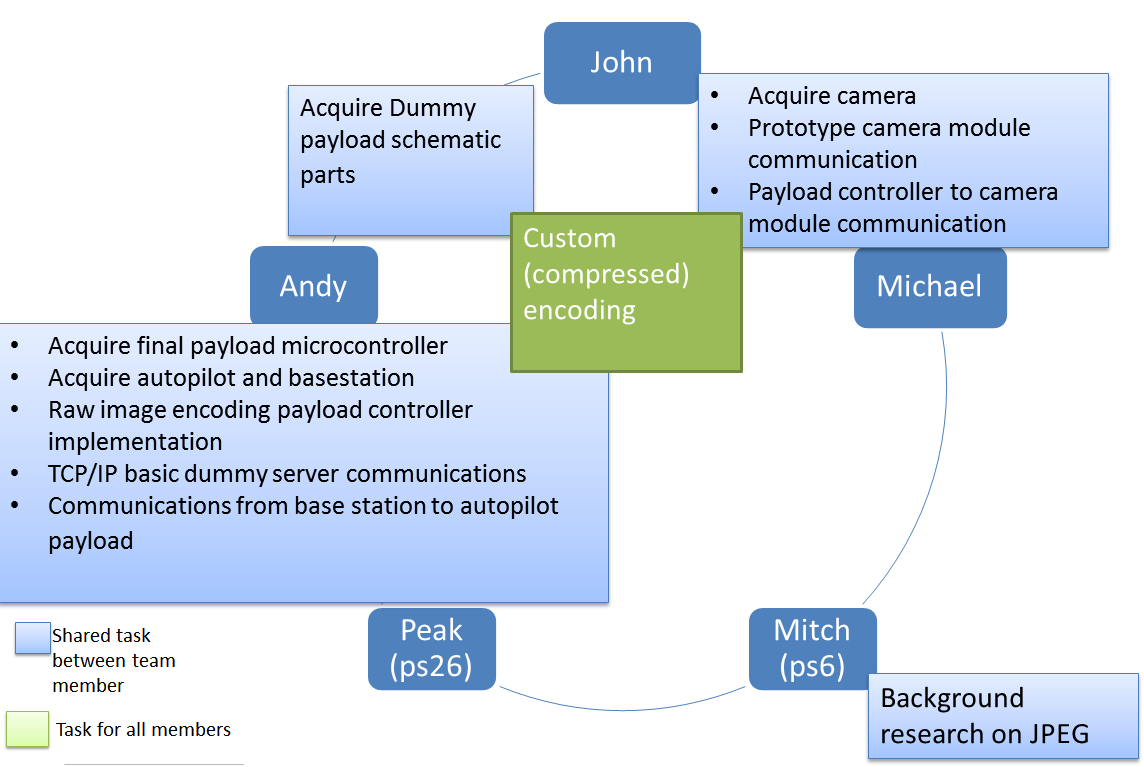
\includegraphics[width=1.0\textwidth]{figures/initial_task_allocation.png} 
\end{center}
\caption{Initial task allocation of the project\label{task allocation}}
\end{figure}

\subsubsection{Schedule - (jc)}
Considerable thought was also given to the scheduling of the tasks, an initial gantt chart was drawn up
at the beginning of the project (see appendix \ref{appendix:gantt}) with a breakdown of the tasks as we
imagined them at the start of the project.

During our regular meetings this gannt chart was used as a gauge for our progress and was ammended when
needed (i.e. our initial timing turned out to be slightly optimistic).
